% !TeX program = xelatex
% ============================================================
% 2014 年·山东卷·文科 · 解析版
% 由 tools/make_editions.py 生成（重跑会覆盖本文件）；
% 题目/解析内容在 questions.tex / answers*.tex，勿在本文件内写内容。
% ============================================================
\documentclass[zihao=-4, a4paper]{ctexart}
% ============================================================
% common/preamble.tex —— 拆分版试卷项目 · 公共导言区
% 引擎：XeLaTeX；文档类 ctexart 由各版本壳文件自行声明
% 由合并书 math-gaokao-2017-2026/preamble.tex 改造而来：
%   - 页眉左右改为可重定义宏 \gkheadL / \gkheadR（各版本壳设置）
%   - hyperref 不再写死 pdftitle（壳内 \hypersetup 覆盖）
%   - 删除书籍专用的 \chaptermark 重定义与 \gkpaper 装配宏
% ============================================================

% ---------- 数学 ----------
\usepackage{amsmath}
\usepackage{amssymb}
\usepackage{mathtools}

% ---------- 绘图 ----------
\usepackage{tikz}
\usetikzlibrary{shapes.geometric, arrows.meta, calc, patterns, angles, quotes, positioning}
\usepackage{pgfplots}
\pgfplotsset{compat=1.18}

% ---------- 版面 ----------
\usepackage{geometry}
\usepackage{needspace}
\geometry{a4paper, margin=2.2cm, headheight=15pt}
% 紧凑版式（如印刷版）可在壳文件中于 \begin{document} 前再次调用 \geometry 覆盖
\usepackage{enumitem}
\setlist{itemsep=2pt, topsep=4pt, parsep=0pt}

% 中文与行内公式混排的断行弹性：
% emergencystretch 允许段落末路不通时追加伸展量；
% 降低二元/关系符罚分，允许行内长公式在 = 、+ 等处断行（否则整段外溢）
\emergencystretch=2em
\binoppenalty=700
\relpenalty=500
\usepackage{booktabs}      % 三线表
\usepackage[most]{tcolorbox}

% ---------- 选择题选项对齐 ----------
% tasks 宏包：\begin{gkopts}(列数) \task ... \end{gkopts}
% 自动等宽分栏，选项天然对齐；列数已由内容片段按选项长度写定（4/2/1）
\usepackage{tasks}
\settasks{label={}, label-width=0pt, item-indent=1.2em,
          column-sep=1em, after-item-skip=2pt, before-skip=2pt, after-skip=4pt}
\NewTasksEnvironment[style=itemize]{gkopts}[\task](4)

% ---------- 页眉页脚 ----------
\newcommand{\gkheadL}{}   % 左页眉：卷名（壳文件 \renewcommand 设置）
\newcommand{\gkheadR}{}   % 右页眉：版本名（壳文件 \renewcommand 设置）
\usepackage{fancyhdr}
\pagestyle{fancy}
\fancyhf{}
\fancyhead[L]{\small\gkheadL}
\fancyhead[R]{\small\gkheadR}
\fancyfoot[C]{\small —— 第 \thepage\ 页 ——}
\renewcommand{\headrulewidth}{0.4pt}

% ---------- 超链接（须最后加载）----------
\usepackage{hyperref}
\hypersetup{colorlinks=true, linkcolor=blue!55!black,
            bookmarksnumbered=true, unicode=true}

% ============================================================
% common/macros.tex —— 自定义命令与环境（题号、解析头、提示框等）
% 与合并书 math-gaokao-2017-2026/preamble.tex 的自定义段保持一致，
% 保证内容片段（questions.tex / answers.tex）在两个项目间可互换。
% ============================================================

% ---------- 试卷标识（壳文件 \renewcommand 设置，用于 label 命名空间）----------
\newcommand{\gkpaperid}{none}

% ---------- 题号 ----------
% 试题部分的题号：加粗编号 + 自动 \label{q:<卷id>:<题号>}
\newcommand{\gkti}[1]{\par\medskip\noindent
  \textbf{#1．}\phantomsection\label{q:\gkpaperid:#1}\ignorespaces}
% 多卷/分部重启题号时，#1 是唯一内部顺序号（交叉引用身份），#2 才是原卷显示题号。
\newcommand{\gktiwithlabel}[2]{\par\medskip\noindent
  \textbf{#2．}\phantomsection\label{q:\gkpaperid:#1}\ignorespaces}

% 解析部分的题头：小标题 + 回链到试题页
% （仅在题目与解析同文档的版本中回链有效；试题版不含解析头，无悬空引用）
\newcommand{\gksolhead}[2]{%
  \Needspace{3\baselineskip}\subsubsection*{第 #1 题\if\relax\detokenize{#2}\relax\else（#2）\fi}%
  \phantomsection\label{s:\gkpaperid:#1}%
  {\small\color{gray}（题目见第~\pageref{q:\gkpaperid:#1}~页）}\par\nopagebreak}
% 与 \gktiwithlabel 成对：显示原题号，但回链仍用唯一内部顺序号。
\newcommand{\gksolheadwithlabel}[3]{%
  \Needspace{3\baselineskip}\subsubsection*{第 #2 题\if\relax\detokenize{#3}\relax\else（#3）\fi}%
  \phantomsection\label{s:\gkpaperid:#1}%
  {\small\color{gray}（题目见第~\pageref{q:\gkpaperid:#1}~页）}\par\nopagebreak}

% ---------- 填空题空位 ----------
\newcommand{\gkblank}{\underline{\hspace{2.2em}}}

% ---------- 提示框 ----------
% 卷种提示 / 解析归属声明（醒目，浅黄）
\newtcolorbox{gknotice}{colback=yellow!8, colframe=orange!60!black,
  boxrule=0.5pt, arc=1.5pt, left=6pt, right=6pt, top=4pt, bottom=4pt,
  before skip=8pt, after skip=8pt}

% 方法提示 / 注（浅蓝，用于解析后的点评与题量说明）
\newtcolorbox{gktip}{colback=blue!4, colframe=blue!35!black,
  boxrule=0.4pt, arc=1.5pt, left=6pt, right=6pt, top=4pt, bottom=4pt,
  before skip=6pt, after skip=6pt, fontupper=\small}

% ---------- 答案行 ----------
% 解析中独立成段的"答案：X"用带底色的行呈现
\newcommand{\gkanswer}[1]{\par\smallskip\noindent
  \tcbox[width=\linewidth, tcbox width=auto limited,
         colback=green!6, colframe=green!35!black, boxrule=0.4pt,
         arc=1.5pt, left=4pt, right=4pt, top=2pt, bottom=2pt,
         nobeforeafter]{\textbf{#1}}\par\smallskip}

% ---------- 结构标题 ----------
% 结构标题后通常紧跟一个带 0.5\textheight 起始预留的解析题块；0.4 只够放标题，
% 会把下一题整体推到下一页，留下孤立的「二、填空题」等页尾标题。
\newcommand{\gkpart}[1]{\Needspace{0.6\textheight}\subsection*{#1}\nopagebreak}     % 标题 + 首题
% （一）必考题 / 解析小问标题：块式加粗段，可自动换行（\paragraph 的 run-in 版式会溢出）
\newcommand{\gksubpart}[1]{\Needspace{6\baselineskip}\par\medskip\noindent\textbf{#1}\par\nopagebreak\smallskip}

% 罗马数字Ⅰ-Ⅻ（U+2160）与圈号①②③（U+2460）划入 CJK 字符类，
% 用中文字体渲染——西文字体 Latin Modern 缺这些字形，否则整段静默丢字
\xeCJKDeclareCharClass{CJK}{"2160 -> "217F, "2460 -> "24FF}

% ============================================================
% common/questions_env.tex —— 题目 / 解析的语义包装环境
%
% questions.tex 中每道题包在 \begin{question}...\end{question} 里，
% answers.tex 中每题解析包在 \begin{answer}...\end{answer} 里；
% 题头排版仍由内容行中的 \gkti / \gksolhead 完成（见 macros.tex）。
%
% 环境本身不产生任何盒子或垂直间距（只引入一个 TeX 分组），
% 排版结果与不包裹时逐点一致。它的价值在于：
%   1. 给每道题一个机器可数的结构边界（校验脚本数环境数 = 题量）；
%   2. 为将来的条件编译留钩子——某版本可重定义环境实现按题取舍。
% ============================================================

% 环境不把整题装盒：题目与解析仍可自然跨页，但开始题块前必须为题面、
% 图形/表格或解析首段留出足够空间。仅保留 2 个 baseline 会让题干、
% 选项和图形在页边界处被拆开，形成不可打印的孤立内容；题目保留
% 0.15\textheight，在避免短题制造大段空白与避免题块拆分之间取平衡。
% 解析题块保留 0.5\textheight，以容纳“题面 + 图形/选项 + 首段解析”；
% 结构标题仍用更大的保留量；末页自然收尾由视觉复审判定。
\newenvironment{question}{\Needspace{0.15\textheight}}{}
\newenvironment{answer}{\Needspace{0.5\textheight}}{}

\renewcommand{\gkpaperid}{gk-2014-shandong-arts}
\renewcommand{\gkheadL}{2014 年·山东卷·文科 · 数学}
\renewcommand{\gkheadR}{解析版}
\hypersetup{pdftitle={2014 年·山东卷·文科 数学 · 解析版}}
\begin{document}
\begin{center}
  {\Large\bfseries 2014 年·山东卷·文科}\\[4pt]
  {\large 数学 · 解析版}
\end{center}
\medskip
\pdfbookmark[1]{试题}{sec:q}
% questions.tex —— 2014 年·山东卷·文科 · 题目内容片段（无答案）
% 由 tools/generate_projects.py 依来源总账自 2014/2014_数学真题_山东文_试题.md 生成，勿手改（改源 MD 后重跑）


\begin{gknotice}
\textbf{来源说明}：本题面依据固定源 PDF 的两页 A3 题面逐题转录，原卷印刷页码为 909—910。第 909 面为选择题 1—10、填空题 11—15 与解答题 16—17；第 910 面为解答题 18—21。全卷三处节头依次为「一、选择题」「二、填空题」「三、解答题」；题号与索引一致。

\textbf{解析归属}：固定源不附答案或解析；配套答案与解析均由本库按本题面独立复算。

\textbf{图形说明}：第 6 题的对数函数图象、第 8 题的频率分布直方图、第 11 题的程序框图、第 18 题的四棱锥由项目内 TikZ 矢量源重绘；其余各题原页无图。
\end{gknotice}

\gkpart{一、选择题}

\begin{question}
\gkti{1}已知 $a,b\in\mathbf R$，$\mathrm i$ 是虚数单位，若 $a+\mathrm i=2-b\mathrm i$，则 $(a+b\mathrm i)^2=$\mbox{（　　）}

（A）$3-4\mathrm i$；（B）$3+4\mathrm i$；（C）$4-3\mathrm i$；（D）$4+3\mathrm i$。

\end{question}
\begin{question}
\gkti{2}设集合 $A=\{x\mid x^2-2x<0\}$，$B=\{x\mid1\leqslant x\leqslant4\}$，则 $A\cap B=$\mbox{（　　）}

（A）$(0,2]$；（B）$(1,2)$；（C）$[1,2)$；（D）$(1,4)$。

\end{question}
\begin{question}
\gkti{3}函数 $f(x)=\dfrac1{\sqrt{\log_2x-1}}$ 的定义域为\mbox{（　　）}

（A）$(0,2)$；（B）$(0,2]$；（C）$(2,+\infty)$；（D）$[2,+\infty)$。

\end{question}
\begin{question}
\gkti{4}用反证法证明命题“设 $a,b$ 为实数，则方程 $x^3+ax+b=0$ 至少有一个实根”时，要做的假设是\mbox{（　　）}

（A）方程 $x^3+ax+b=0$ 没有实根；（B）方程 $x^3+ax+b=0$ 至多有一个实根；（C）方程 $x^3+ax+b=0$ 至多有两个实根；（D）方程 $x^3+ax+b=0$ 恰好有两个实根。

\end{question}
\begin{question}
\gkti{5}已知实数 $x,y$ 满足 $a^x<a^y$（$0<a<1$），则下列关系式恒成立的是\mbox{（　　）}

（A）$x^3>y^3$；（B）$\sin x>\sin y$；（C）$\ln(x^2+1)>\ln(y^2+1)$；（D）$\dfrac1{x^2+1}>\dfrac1{y^2+1}$。

\Needspace{0.4\textheight}
\end{question}
\begin{question}
\gkti{6}已知函数 $y=\log_a(x+c)$（$a,c$ 为常数，其中 $a>0$，$a\neq1$）的图象如图，则下列结论成立的是\mbox{（　　）}

（A）$a>1$，$c>1$；（B）$a>1$，$0<c<1$；（C）$0<a<1$，$c>1$；（D）$0<a<1$，$0<c<1$。
\nopagebreak[4]
\begin{center}% ============================================================
% f2014_shandong_arts_q06_log.tex
% 2014 山东卷（文科）第 6 题：函数 y=log_a(x+c) 的图象
% 来源 PDF：普通高考/2014/2014山东文.pdf
% 原页：第 1 页（A3 横排）左栏，印面 909，第 6 题题干下方
% 特征：图象递减，故 0<a<1；x=0 处函数值为正，故 0<c<1；
%       曲线与 x 轴交点位于 x=1 左侧，即 1-c<1。
% ============================================================
\begin{tikzpicture}[>=Stealth, line width=0.7pt, font=\small,
  x=1cm, y=1cm]

  % 坐标轴
  \draw[->] (-1.35,0) -- (4.95,0) node[below] {$x$};
  \draw[->] (0,-2.55) -- (0,3.05) node[left] {$y$};
  \node[below left] at (0,0) {$O$};

  % 曲线 y=log_{1/2}(x+0.6)，定义域 x>-0.6
  \draw[domain=-0.45:4.75, samples=220, smooth, variable=\x]
    plot ({\x}, {-ln(\x+0.6)/ln(2)});

  % x 轴上的刻度 1
  \draw (1,0.06) -- (1,-0.06);
  \node[above] at (1,0.06) {$1$};

\end{tikzpicture}
\end{center}
\nopagebreak[4]
\end{question}
\begin{question}
\gkti{7}已知向量 $\boldsymbol a=(1,\sqrt3)$，$\boldsymbol b=(3,m)$。若向量 $\boldsymbol a$，$\boldsymbol b$ 的夹角为 $\dfrac\pi6$，则实数 $m=$\mbox{（　　）}

（A）$2\sqrt3$；（B）$\sqrt3$；（C）$0$；（D）$-\sqrt3$。

\Needspace{0.4\textheight}
\end{question}
\begin{question}
\gkti{8}为了研究某种药品的疗效，选取若干名志愿者进行临床试验。所有志愿者的舒张压数据（单位：kPa）的分组区间为 $[12,13)$，$[13,14)$，$[14,15)$，$[15,16)$，$[16,17]$，将其按从左到右的顺序分别编号为第一组，第二组，…，第五组。如图所示是根据试验数据制成的频率分布直方图。已知第一组与第二组共有 $20$ 人，第三组中没有疗效的有 $6$ 人，则第三组中有疗效的人数为\mbox{（　　）}

（A）$6$；（B）$8$；（C）$12$；（D）$18$。
\nopagebreak[4]
\begin{center}% ============================================================
% f2014_shandong_arts_q08_histogram.tex
% 2014 山东卷（文科）第 8 题：舒张压数据的频率分布直方图
% 来源 PDF：普通高考/2014/2014山东文.pdf
% 原页：第 1 页（A3 横排）中栏，印面 909，第 8 题题干右侧
% 各矩形高（频率/组距）：0.24、0.16、0.36、0.16、0.08，和为 1。
% ============================================================
\begin{tikzpicture}[>=Stealth, line width=0.7pt, font=\small,
  x=1cm, y=1cm]

  % 坐标轴
  \draw[->] (0.60,0) -- (7.35,0) node[below right] {舒张压/kPa};
  \draw[->] (0.60,-0.05) -- (0.60,4.05) ;
  \node[below left] at (0.60,0) {$0$};

  % 纵轴标题：频率 / 组距（上下两行，原图无分数线）
  \node at (0.62,4.62) {频率};
  \node at (0.62,4.16) {组距};

  % x 轴断开符号
  \draw (0.86,0) -- (0.98,0.10) -- (1.10,-0.10) -- (1.22,0.10) -- (1.34,0);

  % 直方图：组距 1，映射 12→1.90，13→2.90，…，17→6.90
  \draw (1.90,0) rectangle (2.90,2.40);
  \draw (2.90,0) rectangle (3.90,1.60);
  \draw (3.90,0) rectangle (4.90,3.60);
  \draw (4.90,0) rectangle (5.90,1.60);
  \draw (5.90,0) rectangle (6.90,0.80);

  % 纵轴刻度与虚线
  \foreach \h/\y in {0.08/0.80, 0.16/1.60, 0.24/2.40, 0.36/3.60}
  {
    \draw (0.54,\y) -- (0.66,\y);
    \node[left] at (0.52,\y) {$\h$};
    \draw[dashed] (0.66,\y) -- (6.90,\y);
  }

  % 横轴刻度
  \foreach \x/\l in {1.90/12, 2.90/13, 3.90/14, 4.90/15, 5.90/16, 6.90/17}
  {
    \draw (\x,0.05) -- (\x,-0.05);
    \node[below] at (\x,-0.02) {$\l$};
  }

\end{tikzpicture}
\end{center}
\nopagebreak[4]
\end{question}
\begin{question}
\gkti{9}对于函数 $f(x)$，若存在常数 $a\neq0$，使得 $x$ 取定义域内的每一个值，都有 $f(x)=f(2a-x)$，则称 $f(x)$ 为准偶函数。下列函数中是准偶函数的是\mbox{（　　）}

（A）$f(x)=\sqrt x$；（B）$f(x)=x^3$；（C）$f(x)=\tan x$；（D）$f(x)=\cos(x+1)$。

\end{question}
\begin{question}
\gkti{10}已知 $x,y$ 满足约束条件 $\begin{cases}x-y-1\leqslant0,\\2x-y-3\geqslant0,\end{cases}$ 当目标函数 $z=ax+by$（$a>0$，$b>0$）在该约束条件下取到最小值 $2\sqrt5$ 时，$a^2+b^2$ 的最小值为\mbox{（　　）}

（A）$5$；（B）$4$；（C）$\sqrt5$；（D）$2$。

\end{question}
\gkpart{二、填空题}

\Needspace{0.4\textheight}
\begin{question}
\gkti{11}执行如图所示的程序框图，若输入的 $x$ 的值为 $1$，则输出的 $n$ 的值为\gkblank{}。
\nopagebreak[4]
\begin{center}% ============================================================
% f2014_shandong_arts_q11_flowchart.tex
% 2014 山东卷（文科）第 11 题：程序框图
% 来源 PDF：普通高考/2014/2014山东文.pdf
% 原页：第 1 页（A3 横排）中栏，印面 909，第 11 题题干下方
% 结构：开始 → 输入 x → n=0 → 判断 x^2-4x+3≤0；
%       是：x=x+1 → n=n+1 → 返回判断；否：输出 n → 结束。
% ============================================================
\begin{tikzpicture}[>=Stealth, line width=0.7pt, font=\small,
  x=1cm, y=1cm, line cap=round, line join=round]

  % 开始
  \draw[rounded corners=6pt] (-0.95,0.42) rectangle (0.95,-0.42);
  \node at (0,0) {开始};
  \draw[->] (0,-0.42) -- (0,-0.87);

  % 输入 x
  \draw (-1.45,-0.87) -- (1.45,-0.87) -- (1.25,-1.72) -- (-1.65,-1.72) -- cycle;
  \node at (0,-1.30) {输入 $x$};
  \draw[->] (0,-1.72) -- (0,-2.16);

  % n=0
  \draw (-1.10,-2.16) rectangle (1.10,-2.96);
  \node at (0,-2.56) {$n=0$};
  \draw[->] (0,-2.96) -- (0,-3.45);

  % 判断框
  \draw (0,-3.45) -- (2.55,-4.55) -- (0,-5.65) -- (-2.55,-4.55) -- cycle;
  \node at (0,-4.55) {$x^2-4x+3\leqslant 0$};

  % 是：向下进入循环体
  \draw[->] (0,-5.65) -- (0,-6.10);
  \node at (0.45,-5.90) {是};
  \draw (-1.10,-6.10) rectangle (1.10,-6.90);
  \node at (0,-6.50) {$x=x+1$};

  \draw[->] (0,-6.90) -- (0,-7.35);
  \draw (-1.10,-7.35) rectangle (1.10,-8.15);
  \node at (0,-7.75) {$n=n+1$};

  % 回边：向下、向左、向上，再水平进入判断框左顶点
  \draw[->] (-1.10,-7.75) -- (-3.45,-7.75) -- (-3.45,-4.55) -- (-2.55,-4.55);

  % 否：向右输出
  \draw[->] (2.55,-4.55) -- (3.95,-4.55);
  \node at (3.20,-4.20) {否};
  \draw (3.95,-4.10) -- (6.35,-4.10) -- (6.15,-5.00) -- (3.75,-5.00) -- cycle;
  \node at (5.05,-4.55) {输出 $n$};
  \draw[->] (5.05,-5.00) -- (5.05,-5.45);

  % 结束
  \draw[rounded corners=6pt] (4.10,-5.45) rectangle (6.00,-6.29);
  \node at (5.05,-5.87) {结束};

\end{tikzpicture}
\end{center}
\nopagebreak[4]
\end{question}
\begin{question}
\gkti{12}函数 $y=\dfrac{\sqrt3}2\sin2x+\cos^2x$ 的最小正周期为\gkblank{}。

\end{question}
\begin{question}
\gkti{13}一个六棱锥的体积为 $2\sqrt3$，其底面是边长为 $2$ 的正六边形，侧棱长都相等，则该六棱锥的侧面积为\gkblank{}。

\end{question}
\begin{question}
\gkti{14}圆心在直线 $x-2y=0$ 上的圆 $C$ 与 $y$ 轴的正半轴相切，圆 $C$ 截 $x$ 轴所得弦的长为 $2\sqrt3$，则圆 $C$ 的标准方程为\gkblank{}。

\end{question}
\begin{question}
\gkti{15}已知双曲线 $\dfrac{x^2}{a^2}-\dfrac{y^2}{b^2}=1$（$a>0$，$b>0$）的焦距为 $2c$，右顶点为 $A$，抛物线 $x^2=2py$（$p>0$）的焦点为 $F$。若双曲线截抛物线的准线所得线段长为 $2c$，且 $|FA|=c$，则双曲线的渐近线方程为\gkblank{}。

\end{question}
\gkpart{三、解答题}

\begin{question}
\gkti{16}海关对同时从 $A$，$B$，$C$ 三个不同地区进口的某种商品进行抽样检测，从各地区进口此商品的数量（单位：件）如下表所示。工作人员用分层抽样的方法从这些商品中共抽取 $6$ 件样品进行检测。

\begin{center}
\begin{tabular}{llll}
\toprule
地区 & $A$ & $B$ & $C$ \\
\midrule
数量 & $50$ & $150$ & $100$ \\
\bottomrule
\end{tabular}
\end{center}

（1） 求这 $6$ 件样品中来自 $A$，$B$，$C$ 各地区商品的数量；

（2） 若在这 $6$ 件样品中随机抽取 $2$ 件送往甲机构进行进一步检测，求这 $2$ 件商品来自相同地区的概率。

\end{question}
\begin{question}
\gkti{17}$\triangle ABC$ 中，角 $A$，$B$，$C$ 所对的边分别为 $a$，$b$，$c$。已知 $a=3$，$\cos A=\dfrac{\sqrt6}3$，$B=A+\dfrac\pi2$。

（1） 求 $b$ 的值；

（2） 求 $\triangle ABC$ 的面积。

\Needspace{0.4\textheight}
\end{question}
\begin{question}
\gkti{18}如图，四棱锥 $P-ABCD$ 中，$AP\perp$ 平面 $PCD$，$AD\parallel BC$，$AB=BC=\dfrac12AD$，$E$，$F$ 分别为线段 $AD$，$PC$ 的中点。
\nopagebreak[4]
\begin{center}% ============================================================
% f2014_shandong_arts_q18_pyramid.tex
% 2014 山东卷（文科）第 18 题：四棱锥 P-ABCD
% 来源 PDF：普通高考/2014/2014山东文.pdf
% 原页：第 2 页（A3 横排）左栏，印面 910，第 18 题题干下方
% 结构：AP⊥平面 PCD，AD∥BC，AB=BC=AD/2；
%       E 为 AD 中点，F 为 PC 中点；连 BE、BF、EF，
%       AD、AC 为不可见棱（虚线）。
% ============================================================
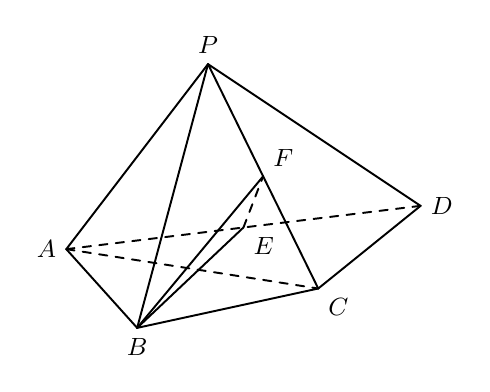
\begin{tikzpicture}[>=Stealth, line width=0.7pt, font=\small,
  x=1cm, y=1cm, line cap=round, line join=round]

  \coordinate (P) at (2.15,3.90);
  \coordinate (A) at (0.35,1.55);
  \coordinate (B) at (1.25,0.55);
  \coordinate (C) at (3.55,1.05);
  \coordinate (D) at (4.85,2.10);

  % 中点
  \coordinate (E) at (2.60,1.825);
  \coordinate (F) at (2.85,2.475);

  % 不可见棱
  \draw[dashed] (A) -- (D);
  \draw[dashed] (A) -- (C);
  \draw[dashed] (E) -- (F);

  % 底面与侧棱
  \draw (P) -- (A);
  \draw (P) -- (B);
  \draw (P) -- (C);
  \draw (P) -- (D);
  \draw (A) -- (B);
  \draw (B) -- (C);
  \draw (C) -- (D);

  % 辅助线
  \draw (B) -- (E);
  \draw (B) -- (F);

  % 顶点标注
  \node[above] at (P) {$P$};
  \node[left] at (A) {$A$};
  \node[below] at (B) {$B$};
  \node[below right] at (C) {$C$};
  \node[right] at (D) {$D$};
  \node[below right] at (E) {$E$};
  \node[above right] at (F) {$F$};

\end{tikzpicture}
\end{center}
\nopagebreak[4]
（1） 求证：$AP\parallel$ 平面 $BEF$；

（2） 求证：$BE\perp$ 平面 $PAC$。

\end{question}
\begin{question}
\gkti{19}在等差数列 $\{a_n\}$ 中，已知公差 $d=2$，$a_2$ 是 $a_1$ 与 $a_4$ 的等比中项。

（1） 求数列 $\{a_n\}$ 的通项公式；

（2） 设 $b_n=a_{\frac{n(n+1)}2}$，记 $T_n=-b_1+b_2-b_3+b_4-\cdots+(-1)^nb_n$，求 $T_n$。

\end{question}
\begin{question}
\gkti{20}设函数 $f(x)=a\ln x+\dfrac{x-1}{x+1}$，其中 $a$ 为常数。

（1） 若 $a=0$，求曲线 $y=f(x)$ 在点 $(1,f(1))$ 处的切线方程；

（2） 讨论函数 $f(x)$ 的单调性。

\end{question}
\begin{question}
\gkti{21}在平面直角坐标系 $xOy$ 中，椭圆 $C:\dfrac{x^2}{a^2}+\dfrac{y^2}{b^2}=1$（$a>b>0$）的离心率为 $\dfrac{\sqrt3}2$，直线 $y=x$ 被椭圆 $C$ 截得的线段长为 $\dfrac{4\sqrt{10}}5$。

（1） 求椭圆 $C$ 的方程；

（2） 过原点的直线与椭圆 $C$ 交于 $A$，$B$ 两点（$A$，$B$ 不是椭圆 $C$ 的顶点）。点 $D$ 在椭圆 $C$ 上，且 $AD\perp AB$，直线 $BD$ 与 $x$ 轴、$y$ 轴分别交于 $M$，$N$ 两点。

　　① 设直线 $BD$，$AM$ 的斜率分别为 $k_1$，$k_2$，证明存在常数 $\lambda$ 使得 $k_1=\lambda k_2$，并求出 $\lambda$ 的值；

　　② 求 $\triangle OMN$ 面积的最大值。

\end{question}
\clearpage
\pdfbookmark[1]{参考答案与详细解析}{sec:s}
\Needspace{8\baselineskip}
\begin{center}{\Large\bfseries 参考答案与详细解析}\end{center}
\medskip
% answers.tex —— 2014 年·山东卷·文科 · 参考答案与详细解析片段
% 由 tools/generate_projects.py 依来源总账自 2014/2014_数学真题_山东文_试题.md + 2014/2014_数学真题_山东文_解析正文.md + 2014/2014_数学真题_山东文_答案要点.md 生成，勿手改（改源 MD 后重跑）


\begin{answer}
\gksolhead{1}{}

\textbf{题目}：

已知 $a,b\in\mathbf R$，$\mathrm i$ 是虚数单位，若 $a+\mathrm i=2-b\mathrm i$，则 $(a+b\mathrm i)^2=$\mbox{（　　）}

（A）$3-4\mathrm i$；（B）$3+4\mathrm i$；（C）$4-3\mathrm i$；（D）$4+3\mathrm i$。

\Needspace{4\baselineskip}
\textbf{解析}

\Needspace{5\baselineskip}
由复数相等的定义，实部与虚部分别相等：
\nopagebreak[4]
\[a=2,\qquad 1=-b,\]
\Needspace{5\baselineskip}
所以 $b=-1$。于是
\nopagebreak[4]
\[(a+b\mathrm i)^2=(2-\mathrm i)^2=4-4\mathrm i+\mathrm i^2=3-4\mathrm i .\]

选 A。

\gkanswer{答案：A。由复数相等得 $a=2$，$b=-1$，故 $(2-\mathrm i)^2=3-4\mathrm i$。}

\end{answer}
\begin{answer}
\gksolhead{2}{}

\textbf{题目}：

设集合 $A=\{x\mid x^2-2x<0\}$，$B=\{x\mid1\leqslant x\leqslant4\}$，则 $A\cap B=$\mbox{（　　）}

（A）$(0,2]$；（B）$(1,2)$；（C）$[1,2)$；（D）$(1,4)$。

\Needspace{4\baselineskip}
\textbf{解析}

\Needspace{5\baselineskip}
先解二次不等式：
\nopagebreak[4]
\[x^2-2x<0\iff x(x-2)<0\iff 0<x<2,\]
\Needspace{5\baselineskip}
即 $A=(0,2)$。又 $B=[1,4]$，在数轴上取交集：
\nopagebreak[4]
\[A\cap B=(0,2)\cap[1,4]=[1,2).\]

选 C。

\gkanswer{答案：C。$x^2-2x<0\iff0<x<2$，与 $B=[1,4]$ 取交得 $[1,2)$。}

\end{answer}
\begin{answer}
\gksolhead{3}{}

\textbf{题目}：

函数 $f(x)=\dfrac1{\sqrt{\log_2x-1}}$ 的定义域为\mbox{（　　）}

（A）$(0,2)$；（B）$(0,2]$；（C）$(2,+\infty)$；（D）$[2,+\infty)$。

\Needspace{4\baselineskip}
\textbf{解析}

\Needspace{5\baselineskip}
根号内为正，且对数的真数为正：
\nopagebreak[4]
\[\begin{cases}x>0,\\[1mm]\log_2x-1>0,\end{cases}
\iff\begin{cases}x>0,\\x>2,\end{cases}\iff x>2 .\]
故定义域为 $(2,+\infty)$。

选 C。

\gkanswer{答案：C。需 $\log_2x-1>0$，即 $x>2$，定义域为 $(2,+\infty)$。}

\end{answer}
\begin{answer}
\gksolhead{4}{}

\textbf{题目}：

用反证法证明命题“设 $a,b$ 为实数，则方程 $x^3+ax+b=0$ 至少有一个实根”时，要做的假设是\mbox{（　　）}

（A）方程 $x^3+ax+b=0$ 没有实根；（B）方程 $x^3+ax+b=0$ 至多有一个实根；（C）方程 $x^3+ax+b=0$ 至多有两个实根；（D）方程 $x^3+ax+b=0$ 恰好有两个实根。

\Needspace{4\baselineskip}
\textbf{解析}

反证法先假设结论的否定。“方程至少有一个实根”的否定是“方程一个实根也没有”，即“方程没有实根”。

选 A。

\gkanswer{答案：A。“至少有一个实根”的否定是“没有实根”。}

\end{answer}
\begin{answer}
\gksolhead{5}{}

\textbf{题目}：

已知实数 $x,y$ 满足 $a^x<a^y$（$0<a<1$），则下列关系式恒成立的是\mbox{（　　）}

（A）$x^3>y^3$；（B）$\sin x>\sin y$；（C）$\ln(x^2+1)>\ln(y^2+1)$；（D）$\dfrac1{x^2+1}>\dfrac1{y^2+1}$。

\Needspace{4\baselineskip}
\textbf{解析}

\Needspace{5\baselineskip}
因为 $0<a<1$，函数 $y=a^x$ 在 $\mathbf R$ 上单调递减，所以
\nopagebreak[4]
\[a^x<a^y\iff x>y .\]
对（A），$y=x^3$ 在 $\mathbf R$ 上严格递增，由 $x>y$ 得 $x^3>y^3$，恒成立。

其余三式均可举出反例：取 $x=\pi$，$y=\dfrac\pi2$，则 $\sin x=0<\sin y=1$，（B）不成立；取 $x=1$，$y=-2$，则 $x^2+1=2<5=y^2+1$，（C）不成立；取 $x=2$，$y=1$，则 $\dfrac1{x^2+1}=\dfrac15<\dfrac12=\dfrac1{y^2+1}$，（D）不成立。

选 A。

\gkanswer{答案：A。由 $0<a<1$ 得 $x>y$，而 $y=x^3$ 在 $\mathbf R$ 上递增，故 $x^3>y^3$ 恒成立；其余各式均可举出反例。}

\end{answer}
\begin{answer}
\gksolhead{6}{}

\textbf{题目}：

已知函数 $y=\log_a(x+c)$（$a,c$ 为常数，其中 $a>0$，$a\neq1$）的图象如图，则下列结论成立的是\mbox{（　　）}

（A）$a>1$，$c>1$；（B）$a>1$，$0<c<1$；（C）$0<a<1$，$c>1$；（D）$0<a<1$，$0<c<1$。
\nopagebreak[4]
\begin{center}% ============================================================
% f2014_shandong_arts_q06_log.tex
% 2014 山东卷（文科）第 6 题：函数 y=log_a(x+c) 的图象
% 来源 PDF：普通高考/2014/2014山东文.pdf
% 原页：第 1 页（A3 横排）左栏，印面 909，第 6 题题干下方
% 特征：图象递减，故 0<a<1；x=0 处函数值为正，故 0<c<1；
%       曲线与 x 轴交点位于 x=1 左侧，即 1-c<1。
% ============================================================
\begin{tikzpicture}[>=Stealth, line width=0.7pt, font=\small,
  x=1cm, y=1cm]

  % 坐标轴
  \draw[->] (-1.35,0) -- (4.95,0) node[below] {$x$};
  \draw[->] (0,-2.55) -- (0,3.05) node[left] {$y$};
  \node[below left] at (0,0) {$O$};

  % 曲线 y=log_{1/2}(x+0.6)，定义域 x>-0.6
  \draw[domain=-0.45:4.75, samples=220, smooth, variable=\x]
    plot ({\x}, {-ln(\x+0.6)/ln(2)});

  % x 轴上的刻度 1
  \draw (1,0.06) -- (1,-0.06);
  \node[above] at (1,0.06) {$1$};

\end{tikzpicture}
\end{center}
\nopagebreak[4]
\Needspace{4\baselineskip}
\textbf{解析}

\Needspace{5\baselineskip}
由图象，函数随 $x$ 增大而下降，故底数满足
\nopagebreak[4]
\[0<a<1 .\]
\Needspace{5\baselineskip}
图象与 $y$ 轴有交点，故 $x=0$ 在定义域内，即 $c>0$。在该点函数值在 $x$ 轴上方：
\nopagebreak[4]
\[\log_ac>0 .\]
\Needspace{5\baselineskip}
当 $0<a<1$ 时，$\log_at>0\iff0<t<1$，故
\nopagebreak[4]
\[0<c<1 .\]
（这与图象和 $x$ 轴的交点 $x=1-c\in(0,1)$ 位于 $x=1$ 左侧一致。）

选 D。

\gkanswer{答案：D。图象递减故 $0<a<1$；$x=0$ 时函数值为正，即 $\log_ac>0$，故 $0<c<1$。}

\end{answer}
\begin{answer}
\gksolhead{7}{}

\textbf{题目}：

已知向量 $\boldsymbol a=(1,\sqrt3)$，$\boldsymbol b=(3,m)$。若向量 $\boldsymbol a$，$\boldsymbol b$ 的夹角为 $\dfrac\pi6$，则实数 $m=$\mbox{（　　）}

（A）$2\sqrt3$；（B）$\sqrt3$；（C）$0$；（D）$-\sqrt3$。

\Needspace{4\baselineskip}
\textbf{解析}

\Needspace{5\baselineskip}
先算数量积与模：
\nopagebreak[4]
\[\boldsymbol a\cdot\boldsymbol b=1\times3+\sqrt3\,m=3+\sqrt3m,\qquad
|\boldsymbol a|=\sqrt{1+3}=2,\qquad
|\boldsymbol b|=\sqrt{9+m^2}.\]
\Needspace{5\baselineskip}
由夹角公式
\nopagebreak[4]
\[\cos\frac\pi6=\frac{\boldsymbol a\cdot\boldsymbol b}{|\boldsymbol a||\boldsymbol b|}
=\frac{3+\sqrt3m}{2\sqrt{9+m^2}}=\frac{\sqrt3}2 .\]
\Needspace{5\baselineskip}
即
\nopagebreak[4]
\[3+\sqrt3m=\sqrt3\sqrt{9+m^2}.\]
\Needspace{5\baselineskip}
两边平方：
\nopagebreak[4]
\[9+6\sqrt3m+3m^2=3(9+m^2)=27+3m^2,\]
\Needspace{5\baselineskip}
所以
\nopagebreak[4]
\[6\sqrt3m=18\Longrightarrow m=\sqrt3 .\]
代回检验：$3+\sqrt3\cdot\sqrt3=6>0$，符合。

选 B。

\gkanswer{答案：B。由 $\dfrac{3+\sqrt3m}{2\sqrt{9+m^2}}=\dfrac{\sqrt3}2$ 平方解得 $m=\sqrt3$（另一根不合）。}

\end{answer}
\begin{answer}
\gksolhead{8}{}

\textbf{题目}：

为了研究某种药品的疗效，选取若干名志愿者进行临床试验。所有志愿者的舒张压数据（单位：kPa）的分组区间为 $[12,13)$，$[13,14)$，$[14,15)$，$[15,16)$，$[16,17]$，将其按从左到右的顺序分别编号为第一组，第二组，…，第五组。如图所示是根据试验数据制成的频率分布直方图。已知第一组与第二组共有 $20$ 人，第三组中没有疗效的有 $6$ 人，则第三组中有疗效的人数为\mbox{（　　）}

（A）$6$；（B）$8$；（C）$12$；（D）$18$。
\nopagebreak[4]
\begin{center}% ============================================================
% f2014_shandong_arts_q08_histogram.tex
% 2014 山东卷（文科）第 8 题：舒张压数据的频率分布直方图
% 来源 PDF：普通高考/2014/2014山东文.pdf
% 原页：第 1 页（A3 横排）中栏，印面 909，第 8 题题干右侧
% 各矩形高（频率/组距）：0.24、0.16、0.36、0.16、0.08，和为 1。
% ============================================================
\begin{tikzpicture}[>=Stealth, line width=0.7pt, font=\small,
  x=1cm, y=1cm]

  % 坐标轴
  \draw[->] (0.60,0) -- (7.35,0) node[below right] {舒张压/kPa};
  \draw[->] (0.60,-0.05) -- (0.60,4.05) ;
  \node[below left] at (0.60,0) {$0$};

  % 纵轴标题：频率 / 组距（上下两行，原图无分数线）
  \node at (0.62,4.62) {频率};
  \node at (0.62,4.16) {组距};

  % x 轴断开符号
  \draw (0.86,0) -- (0.98,0.10) -- (1.10,-0.10) -- (1.22,0.10) -- (1.34,0);

  % 直方图：组距 1，映射 12→1.90，13→2.90，…，17→6.90
  \draw (1.90,0) rectangle (2.90,2.40);
  \draw (2.90,0) rectangle (3.90,1.60);
  \draw (3.90,0) rectangle (4.90,3.60);
  \draw (4.90,0) rectangle (5.90,1.60);
  \draw (5.90,0) rectangle (6.90,0.80);

  % 纵轴刻度与虚线
  \foreach \h/\y in {0.08/0.80, 0.16/1.60, 0.24/2.40, 0.36/3.60}
  {
    \draw (0.54,\y) -- (0.66,\y);
    \node[left] at (0.52,\y) {$\h$};
    \draw[dashed] (0.66,\y) -- (6.90,\y);
  }

  % 横轴刻度
  \foreach \x/\l in {1.90/12, 2.90/13, 3.90/14, 4.90/15, 5.90/16, 6.90/17}
  {
    \draw (\x,0.05) -- (\x,-0.05);
    \node[below] at (\x,-0.02) {$\l$};
  }

\end{tikzpicture}
\end{center}
\nopagebreak[4]
\Needspace{4\baselineskip}
\textbf{解析}

\Needspace{5\baselineskip}
组距为 $1$，故各矩形的面积等于相应频率。五组矩形的高依次为
\nopagebreak[4]
\[0.24,\quad0.16,\quad0.36,\quad0.16,\quad0.08,\]
\Needspace{5\baselineskip}
其和为 $1$，与频率之和为 $1$ 一致。第一组与第二组的频率之和为
\nopagebreak[4]
\[0.24+0.16=0.40,\]
\Needspace{5\baselineskip}
对应 $20$ 人，故总人数
\nopagebreak[4]
\[N=\frac{20}{0.40}=50 .\]
\Needspace{5\baselineskip}
第三组的频率为 $0.36$，人数为
\nopagebreak[4]
\[0.36\times50=18 .\]
\Needspace{5\baselineskip}
其中没有疗效的有 $6$ 人，故有疗效的人数为
\nopagebreak[4]
\[18-6=12 .\]

选 C。

\gkanswer{答案：C。前两组频率和为 $0.40$，故总人数 $50$；第三组 $0.36\times50=18$ 人，减去无疗效的 $6$ 人得 $12$。}

\end{answer}
\begin{answer}
\gksolhead{9}{}

\textbf{题目}：

对于函数 $f(x)$，若存在常数 $a\neq0$，使得 $x$ 取定义域内的每一个值，都有 $f(x)=f(2a-x)$，则称 $f(x)$ 为准偶函数。下列函数中是准偶函数的是\mbox{（　　）}

（A）$f(x)=\sqrt x$；（B）$f(x)=x^3$；（C）$f(x)=\tan x$；（D）$f(x)=\cos(x+1)$。

\Needspace{4\baselineskip}
\textbf{解析}

条件 $f(x)=f(2a-x)$ 表示函数图象关于直线 $x=a$ 对称（点 $x$ 与 $2a-x$ 关于 $x=a$ 对称）。

（A）$\sqrt x$ 的定义域为 $[0,+\infty)$，不关于任何 $x=a$（$a\neq0$）对称；

（B）$x^3$ 为奇函数，图象关于原点对称，没有竖直对称轴；

（C）$\tan x$ 在每个连续区间上严格单调，没有竖直对称轴；

\Needspace{5\baselineskip}
（D）取 $a=-1$，则
\nopagebreak[4]
\[f(2a-x)=\cos\bigl(2\cdot(-1)-x+1\bigr)=\cos(-1-x)=\cos(x+1)=f(x),\]
故 $\cos(x+1)$ 是准偶函数。

选 D。

\gkanswer{答案：D。$f(x)=f(2a-x)$ 表示图象关于直线 $x=a$ 对称，$\cos(x+1)$ 关于 $x=-1$ 对称，取 $a=-1\neq0$。}

\end{answer}
\begin{answer}
\gksolhead{10}{}

\textbf{题目}：

已知 $x,y$ 满足约束条件 $\begin{cases}x-y-1\leqslant0,\\2x-y-3\geqslant0,\end{cases}$ 当目标函数 $z=ax+by$（$a>0$，$b>0$）在该约束条件下取到最小值 $2\sqrt5$ 时，$a^2+b^2$ 的最小值为\mbox{（　　）}

（A）$5$；（B）$4$；（C）$\sqrt5$；（D）$2$。

\Needspace{4\baselineskip}
\textbf{解析}

\Needspace{5\baselineskip}
约束条件即
\nopagebreak[4]
\[x-1\leqslant y\leqslant2x-3,\]
两边界相交于 $(2,1)$，且需 $x\geqslant2$。可行域是顶点为 $(2,1)$、向右侧无限延伸的角形区域。

\Needspace{5\baselineskip}
由 $y\geqslant x-1$ 及 $a>0$，$b>0$，
\nopagebreak[4]
\[z=ax+by\geqslant ax+b(x-1)=(a+b)x-b\geqslant2(a+b)-b=2a+b,\]
\Needspace{5\baselineskip}
等号在顶点 $(2,1)$ 处取得。故
\nopagebreak[4]
\[z_{\min}=2a+b=2\sqrt5 .\]
\Needspace{5\baselineskip}
由柯西不等式
\nopagebreak[4]
\[(2^2+1^2)(a^2+b^2)\geqslant(2a+b)^2=20,\]
\Needspace{5\baselineskip}
得
\nopagebreak[4]
\[a^2+b^2\geqslant4 .\]
等号当 $\dfrac a2=\dfrac b1$，结合 $2a+b=2\sqrt5$ 得 $a=\dfrac{4\sqrt5}5$，$b=\dfrac{2\sqrt5}5$，可以取得。

选 B。

\gkanswer{答案：B。可行域顶点 $(2,1)$ 处取最小值，故 $2a+b=2\sqrt5$；由柯西不等式 $5(a^2+b^2)\geqslant(2a+b)^2=20$，得 $a^2+b^2\geqslant4$。}

\end{answer}
\begin{answer}
\gksolhead{11}{}

\textbf{题目}：

执行如图所示的程序框图，若输入的 $x$ 的值为 $1$，则输出的 $n$ 的值为\gkblank{}。
\nopagebreak[4]
\begin{center}% ============================================================
% f2014_shandong_arts_q11_flowchart.tex
% 2014 山东卷（文科）第 11 题：程序框图
% 来源 PDF：普通高考/2014/2014山东文.pdf
% 原页：第 1 页（A3 横排）中栏，印面 909，第 11 题题干下方
% 结构：开始 → 输入 x → n=0 → 判断 x^2-4x+3≤0；
%       是：x=x+1 → n=n+1 → 返回判断；否：输出 n → 结束。
% ============================================================
\begin{tikzpicture}[>=Stealth, line width=0.7pt, font=\small,
  x=1cm, y=1cm, line cap=round, line join=round]

  % 开始
  \draw[rounded corners=6pt] (-0.95,0.42) rectangle (0.95,-0.42);
  \node at (0,0) {开始};
  \draw[->] (0,-0.42) -- (0,-0.87);

  % 输入 x
  \draw (-1.45,-0.87) -- (1.45,-0.87) -- (1.25,-1.72) -- (-1.65,-1.72) -- cycle;
  \node at (0,-1.30) {输入 $x$};
  \draw[->] (0,-1.72) -- (0,-2.16);

  % n=0
  \draw (-1.10,-2.16) rectangle (1.10,-2.96);
  \node at (0,-2.56) {$n=0$};
  \draw[->] (0,-2.96) -- (0,-3.45);

  % 判断框
  \draw (0,-3.45) -- (2.55,-4.55) -- (0,-5.65) -- (-2.55,-4.55) -- cycle;
  \node at (0,-4.55) {$x^2-4x+3\leqslant 0$};

  % 是：向下进入循环体
  \draw[->] (0,-5.65) -- (0,-6.10);
  \node at (0.45,-5.90) {是};
  \draw (-1.10,-6.10) rectangle (1.10,-6.90);
  \node at (0,-6.50) {$x=x+1$};

  \draw[->] (0,-6.90) -- (0,-7.35);
  \draw (-1.10,-7.35) rectangle (1.10,-8.15);
  \node at (0,-7.75) {$n=n+1$};

  % 回边：向下、向左、向上，再水平进入判断框左顶点
  \draw[->] (-1.10,-7.75) -- (-3.45,-7.75) -- (-3.45,-4.55) -- (-2.55,-4.55);

  % 否：向右输出
  \draw[->] (2.55,-4.55) -- (3.95,-4.55);
  \node at (3.20,-4.20) {否};
  \draw (3.95,-4.10) -- (6.35,-4.10) -- (6.15,-5.00) -- (3.75,-5.00) -- cycle;
  \node at (5.05,-4.55) {输出 $n$};
  \draw[->] (5.05,-5.00) -- (5.05,-5.45);

  % 结束
  \draw[rounded corners=6pt] (4.10,-5.45) rectangle (6.00,-6.29);
  \node at (5.05,-5.87) {结束};

\end{tikzpicture}
\end{center}
\nopagebreak[4]
\Needspace{4\baselineskip}
\textbf{解析}

初值 $x=1$，$n=0$。每轮判断 $x^2-4x+3\leqslant0$：成立则 $x$ 增 $1$、$n$ 增 $1$ 后返回；不成立则输出 $n$。

\begin{center}
\begin{tabular}{lllll}
\toprule
轮次 & 判断前 $x$ & $x^2-4x+3$ & 是否 $\leqslant0$ & 执行后 $(x,n)$ \\
\midrule
1 & $1$ & $0$ & 是 & $(2,1)$ \\
2 & $2$ & $-1$ & 是 & $(3,2)$ \\
3 & $3$ & $0$ & 是 & $(4,3)$ \\
4 & $4$ & $3$ & 否 & 输出 $n=3$ \\
\bottomrule
\end{tabular}
\end{center}

故输出的 $n$ 的值为 $3$。

\gkanswer{答案：$3$。$x=1,2,3$ 时条件成立，依次得 $n=1,2,3$；$x=4$ 时 $3>0$ 不成立，输出 $n=3$。}

\end{answer}
\begin{answer}
\gksolhead{12}{}

\textbf{题目}：

函数 $y=\dfrac{\sqrt3}2\sin2x+\cos^2x$ 的最小正周期为\gkblank{}。

\Needspace{4\baselineskip}
\textbf{解析}

\Needspace{5\baselineskip}
用二倍角公式降幂：
\nopagebreak[4]
\[y=\frac{\sqrt3}2\sin2x+\frac{1+\cos2x}2
=\frac{\sqrt3}2\sin2x+\frac12\cos2x+\frac12 .\]
\Needspace{5\baselineskip}
由辅助角公式
\nopagebreak[4]
\[\frac{\sqrt3}2\sin2x+\frac12\cos2x=\sin\left(2x+\frac\pi6\right),\]
\Needspace{5\baselineskip}
故
\nopagebreak[4]
\[y=\sin\left(2x+\frac\pi6\right)+\frac12 .\]
\Needspace{5\baselineskip}
最小正周期
\nopagebreak[4]
\[T=\frac{2\pi}2=\pi .\]

\gkanswer{答案：$\pi$。$y=\sin\left(2x+\dfrac\pi6\right)+\dfrac12$，最小正周期为 $\dfrac{2\pi}2=\pi$。}

\end{answer}
\begin{answer}
\gksolhead{13}{}

\textbf{题目}：

一个六棱锥的体积为 $2\sqrt3$，其底面是边长为 $2$ 的正六边形，侧棱长都相等，则该六棱锥的侧面积为\gkblank{}。

\Needspace{4\baselineskip}
\textbf{解析}

\Needspace{5\baselineskip}
底面是边长为 $2$ 的正六边形，面积
\nopagebreak[4]
\[S_{\text{\text{底}}}=6\cdot\frac{\sqrt3}4\cdot2^2=6\sqrt3 .\]
\Needspace{5\baselineskip}
设棱锥的高为 $h$。由体积
\nopagebreak[4]
\[V=\frac13S_{\text{\text{底}}}h=\frac13\cdot6\sqrt3\cdot h=2\sqrt3,\]
得 $h=1$。

\Needspace{5\baselineskip}
侧棱长都相等，故顶点在底面中心的正上方。底面正六边形的边心距
\nopagebreak[4]
\[r=\frac{\sqrt3}2\times2=\sqrt3,\]
\Needspace{5\baselineskip}
斜高
\nopagebreak[4]
\[l=\sqrt{h^2+r^2}=\sqrt{1+3}=2 .\]
\Needspace{5\baselineskip}
每个侧面是底边 $2$、斜高 $2$ 的等腰三角形，故侧面积
\nopagebreak[4]
\[S_{\text{\text{侧}}}=6\cdot\frac12\cdot2\cdot2=12 .\]

\gkanswer{答案：$12$。底面积 $6\sqrt3$，由 $V=2\sqrt3$ 得高 $h=1$；底面边心距 $\sqrt3$，斜高 $2$，侧面积 $6\times\dfrac12\times2\times2=12$。}

\end{answer}
\begin{answer}
\gksolhead{14}{}

\textbf{题目}：

圆心在直线 $x-2y=0$ 上的圆 $C$ 与 $y$ 轴的正半轴相切，圆 $C$ 截 $x$ 轴所得弦的长为 $2\sqrt3$，则圆 $C$ 的标准方程为\gkblank{}。

\Needspace{4\baselineskip}
\textbf{解析}

\Needspace{5\baselineskip}
圆心在 $x-2y=0$ 上，设圆心 $C(2t,t)$。圆与 $y$ 轴正半轴相切，故 $t>0$，且半径等于圆心到 $y$ 轴的距离：
\nopagebreak[4]
\[r=2t .\]
\Needspace{5\baselineskip}
圆心到 $x$ 轴的距离为 $t$。圆截 $x$ 轴所得弦长为 $2\sqrt3$，半弦长为 $\sqrt3$，由勾股关系
\nopagebreak[4]
\[r^2=t^2+(\sqrt3)^2\Longrightarrow4t^2=t^2+3\Longrightarrow t^2=1 .\]
\Needspace{5\baselineskip}
由 $t>0$ 得 $t=1$，故圆心 $(2,1)$，半径 $r=2$，标准方程为
\nopagebreak[4]
\[(x-2)^2+(y-1)^2=4 .\]

\gkanswer{答案：$(x-2)^2+(y-1)^2=4$。设圆心 $(2t,t)$、半径 $2t$，由 $4t^2=t^2+3$ 得 $t=1$。}

\end{answer}
\begin{answer}
\gksolhead{15}{}

\textbf{题目}：

已知双曲线 $\dfrac{x^2}{a^2}-\dfrac{y^2}{b^2}=1$（$a>0$，$b>0$）的焦距为 $2c$，右顶点为 $A$，抛物线 $x^2=2py$（$p>0$）的焦点为 $F$。若双曲线截抛物线的准线所得线段长为 $2c$，且 $|FA|=c$，则双曲线的渐近线方程为\gkblank{}。

\Needspace{4\baselineskip}
\textbf{解析}

\Needspace{5\baselineskip}
抛物线 $x^2=2py$ 的准线为 $y=-\dfrac p2$。将其代入双曲线：
\nopagebreak[4]
\[\frac{x^2}{a^2}-\frac{p^2}{4b^2}=1
\Longrightarrow x^2=a^2\left(1+\frac{p^2}{4b^2}\right),\]
\Needspace{5\baselineskip}
故截得线段长为
\nopagebreak[4]
\[2a\sqrt{1+\frac{p^2}{4b^2}}=2c
\Longrightarrow a^2\left(1+\frac{p^2}{4b^2}\right)=c^2.\]

\Needspace{5\baselineskip}
又 $F\left(0,\dfrac p2\right)$，$A(a,0)$，由 $|FA|=c$：
\nopagebreak[4]
\[a^2+\frac{p^2}4=c^2
\Longrightarrow\frac{p^2}4=c^2-a^2=b^2 .\]
\Needspace{5\baselineskip}
将 $\dfrac{p^2}4=b^2$ 代入前一式：
\nopagebreak[4]
\[a^2\left(1+\frac{b^2}{b^2}\right)=2a^2=c^2
\Longrightarrow c^2=2a^2 .\]
\Needspace{5\baselineskip}
于是
\nopagebreak[4]
\[b^2=c^2-a^2=a^2\Longrightarrow b=a .\]
\Needspace{5\baselineskip}
渐近线方程为
\nopagebreak[4]
\[y=\pm\frac bax=\pm x .\]

\gkanswer{答案：$y=\pm x$。由 $|FA|=c$ 得 $\dfrac{p^2}4=b^2$，再由准线截得弦长 $2c$ 得 $c^2=2a^2$，故 $b=a$。}

\end{answer}
\begin{answer}
\gksolhead{16}{}

\textbf{题目}：

海关对同时从 $A$，$B$，$C$ 三个不同地区进口的某种商品进行抽样检测，从各地区进口此商品的数量（单位：件）如下表所示。工作人员用分层抽样的方法从这些商品中共抽取 $6$ 件样品进行检测。

\begin{center}
\begin{tabular}{llll}
\toprule
地区 & $A$ & $B$ & $C$ \\
\midrule
数量 & $50$ & $150$ & $100$ \\
\bottomrule
\end{tabular}
\end{center}

（1） 求这 $6$ 件样品中来自 $A$，$B$，$C$ 各地区商品的数量；

（2） 若在这 $6$ 件样品中随机抽取 $2$ 件送往甲机构进行进一步检测，求这 $2$ 件商品来自相同地区的概率。

\Needspace{4\baselineskip}
\textbf{解析}

\Needspace{5\baselineskip}
\textbf{（1）} 三地区商品总数为
\nopagebreak[4]
\[50+150+100=300 .\]
\Needspace{5\baselineskip}
样本量为 $6$，抽样比为
\nopagebreak[4]
\[\frac6{300}=\frac1{50}.\]
\Needspace{5\baselineskip}
故各地区抽取数量为
\nopagebreak[4]
\[A:\ 50\times\frac1{50}=1,\qquad
B:\ 150\times\frac1{50}=3,\qquad
C:\ 100\times\frac1{50}=2 .\]
即 $A$ 地区 $1$ 件，$B$ 地区 $3$ 件，$C$ 地区 $2$ 件。

\Needspace{5\baselineskip}
\textbf{（2）} 从 $6$ 件中任取 $2$ 件的取法数为
\nopagebreak[4]
\[\mathrm C_6^2=15 .\]
\Needspace{5\baselineskip}
两件来自相同地区，可按地区分三类：
\nopagebreak[4]
\[\mathrm C_1^2+\mathrm C_3^2+\mathrm C_2^2=0+3+1=4 .\]
\Needspace{5\baselineskip}
故所求概率
\nopagebreak[4]
\[P=\frac4{15}.\]

\gkanswer{答案（1）：$A$ 地区 $1$ 件，$B$ 地区 $3$ 件，$C$ 地区 $2$ 件。三层数量之比为 $1:3:2$，共抽 $6$ 件。}

\gkanswer{答案（2）：$\dfrac4{15}$。$\dfrac{\mathrm C_1^2+\mathrm C_3^2+\mathrm C_2^2}{\mathrm C_6^2}=\dfrac{0+3+1}{15}=\dfrac4{15}$。}

\end{answer}
\begin{answer}
\gksolhead{17}{}

\textbf{题目}：

$\triangle ABC$ 中，角 $A$，$B$，$C$ 所对的边分别为 $a$，$b$，$c$。已知 $a=3$，$\cos A=\dfrac{\sqrt6}3$，$B=A+\dfrac\pi2$。

（1） 求 $b$ 的值；

（2） 求 $\triangle ABC$ 的面积。

\Needspace{4\baselineskip}
\textbf{解析}

\Needspace{5\baselineskip}
\textbf{（1）} 由 $B=A+\dfrac\pi2$ 得
\nopagebreak[4]
\[\sin B=\sin\left(A+\frac\pi2\right)=\cos A=\frac{\sqrt6}3 .\]
\Needspace{5\baselineskip}
因为 $\cos A>0$，$A$ 为锐角，所以
\nopagebreak[4]
\[\sin A=\sqrt{1-\cos^2A}=\sqrt{1-\frac69}=\frac{\sqrt3}3 .\]
\Needspace{5\baselineskip}
由正弦定理 $\dfrac b{\sin B}=\dfrac a{\sin A}$，
\nopagebreak[4]
\[b=a\cdot\frac{\sin B}{\sin A}
=3\cdot\frac{\sqrt6/3}{\sqrt3/3}=3\sqrt2 .\]

\Needspace{5\baselineskip}
\textbf{（2）} 由内角和
\nopagebreak[4]
\[C=\pi-A-B=\pi-A-\left(A+\frac\pi2\right)=\frac\pi2-2A .\]
\Needspace{5\baselineskip}
于是
\nopagebreak[4]
\[\sin C=\sin\left(\frac\pi2-2A\right)=\cos2A=2\cos^2A-1
=2\cdot\frac69-1=\frac13 .\]
\Needspace{5\baselineskip}
故
\nopagebreak[4]
\[S_{\triangle ABC}=\frac12ab\sin C
=\frac12\cdot3\cdot3\sqrt2\cdot\frac13
=\frac{3\sqrt2}2 .\]

\gkanswer{答案（1）：$b=3\sqrt2$。$\sin B=\cos A=\dfrac{\sqrt6}3$，$\sin A=\dfrac{\sqrt3}3$，由正弦定理得 $b=3\sqrt2$。}

\gkanswer{答案（2）：$\dfrac{3\sqrt2}2$。$C=\dfrac\pi2-2A$，$\sin C=\cos2A=\dfrac13$，故 $S=\dfrac12ab\sin C=\dfrac{3\sqrt2}2$。}

\end{answer}
\begin{answer}
\gksolhead{18}{}

\textbf{题目}：

如图，四棱锥 $P-ABCD$ 中，$AP\perp$ 平面 $PCD$，$AD\parallel BC$，$AB=BC=\dfrac12AD$，$E$，$F$ 分别为线段 $AD$，$PC$ 的中点。
\nopagebreak[4]
\begin{center}% ============================================================
% f2014_shandong_arts_q18_pyramid.tex
% 2014 山东卷（文科）第 18 题：四棱锥 P-ABCD
% 来源 PDF：普通高考/2014/2014山东文.pdf
% 原页：第 2 页（A3 横排）左栏，印面 910，第 18 题题干下方
% 结构：AP⊥平面 PCD，AD∥BC，AB=BC=AD/2；
%       E 为 AD 中点，F 为 PC 中点；连 BE、BF、EF，
%       AD、AC 为不可见棱（虚线）。
% ============================================================
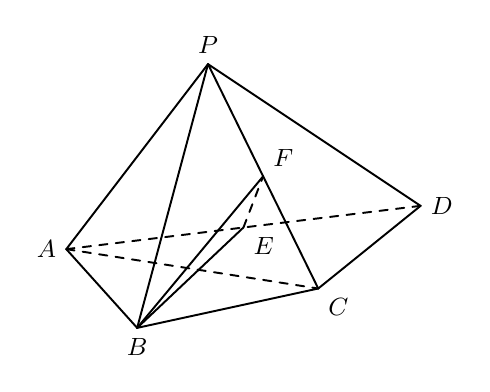
\begin{tikzpicture}[>=Stealth, line width=0.7pt, font=\small,
  x=1cm, y=1cm, line cap=round, line join=round]

  \coordinate (P) at (2.15,3.90);
  \coordinate (A) at (0.35,1.55);
  \coordinate (B) at (1.25,0.55);
  \coordinate (C) at (3.55,1.05);
  \coordinate (D) at (4.85,2.10);

  % 中点
  \coordinate (E) at (2.60,1.825);
  \coordinate (F) at (2.85,2.475);

  % 不可见棱
  \draw[dashed] (A) -- (D);
  \draw[dashed] (A) -- (C);
  \draw[dashed] (E) -- (F);

  % 底面与侧棱
  \draw (P) -- (A);
  \draw (P) -- (B);
  \draw (P) -- (C);
  \draw (P) -- (D);
  \draw (A) -- (B);
  \draw (B) -- (C);
  \draw (C) -- (D);

  % 辅助线
  \draw (B) -- (E);
  \draw (B) -- (F);

  % 顶点标注
  \node[above] at (P) {$P$};
  \node[left] at (A) {$A$};
  \node[below] at (B) {$B$};
  \node[below right] at (C) {$C$};
  \node[right] at (D) {$D$};
  \node[below right] at (E) {$E$};
  \node[above right] at (F) {$F$};

\end{tikzpicture}
\end{center}
\nopagebreak[4]
（1） 求证：$AP\parallel$ 平面 $BEF$；

（2） 求证：$BE\perp$ 平面 $PAC$。

\Needspace{4\baselineskip}
\textbf{解析}

\textbf{（1）} 取 $PD$ 的中点 $G$，连接 $FG$，$EG$。

\Needspace{5\baselineskip}
在 $\triangle PCD$ 中，$F$，$G$ 分别为 $PC$，$PD$ 的中点，由中位线定理
\nopagebreak[4]
\[FG\parallel CD,\qquad FG=\frac12CD .\]
\Needspace{5\baselineskip}
又 $AD\parallel BC$ 且 $AD=2BC$，$E$ 为 $AD$ 的中点，故
\nopagebreak[4]
\[ED=\frac12AD=BC,\qquad ED\parallel BC,\]
\Needspace{5\baselineskip}
所以四边形 $BCDE$ 是平行四边形，从而
\nopagebreak[4]
\[BE\parallel CD,\qquad BE=CD .\]
于是 $FG\parallel BE$，两条平行直线确定一个平面，即 $B$，$E$，$F$，$G$ 四点共面，所以 $G\in$ 平面 $BEF$。

\Needspace{5\baselineskip}
在 $\triangle PAD$ 中，$E$，$G$ 分别为 $AD$，$PD$ 的中点，故
\nopagebreak[4]
\[EG\parallel AP .\]
\Needspace{5\baselineskip}
又 $EG\subset$ 平面 $BEF$，而 $AP\not\subset$ 平面 $BEF$，由线面平行的判定定理
\nopagebreak[4]
\[AP\parallel\text{\text{平面} }BEF .\]

\Needspace{5\baselineskip}
\textbf{（2）} 由 $AD\parallel BC$ 及 $AE=\dfrac12AD=BC$ 得 $AE\parallel BC$ 且 $AE=BC$，故四边形 $ABCE$ 是平行四边形。又 $AB=BC$，所以 $ABCE$ 是菱形，其对角线互相垂直：
\nopagebreak[4]
\[AC\perp BE .\]

\Needspace{5\baselineskip}
由（1）知 $BE\parallel CD$。因为 $AP\perp$ 平面 $PCD$，而 $CD\subset$ 平面 $PCD$，所以
\nopagebreak[4]
\[AP\perp CD,\]
\Needspace{5\baselineskip}
从而
\nopagebreak[4]
\[AP\perp BE .\]

\Needspace{5\baselineskip}
又 $AC\cap AP=A$，且 $AC$，$AP$ 都在平面 $PAC$ 内，由线面垂直的判定定理
\nopagebreak[4]
\[BE\perp\text{\text{平面} }PAC .\]

\gkanswer{答案（1）：见解析版}

\gkanswer{答案（2）：见解析版}

\end{answer}
\begin{answer}
\gksolhead{19}{}

\textbf{题目}：

在等差数列 $\{a_n\}$ 中，已知公差 $d=2$，$a_2$ 是 $a_1$ 与 $a_4$ 的等比中项。

（1） 求数列 $\{a_n\}$ 的通项公式；

（2） 设 $b_n=a_{\frac{n(n+1)}2}$，记 $T_n=-b_1+b_2-b_3+b_4-\cdots+(-1)^nb_n$，求 $T_n$。

\Needspace{4\baselineskip}
\textbf{解析}

\Needspace{5\baselineskip}
\textbf{（1）} 由公差 $d=2$ 得
\nopagebreak[4]
\[a_2=a_1+2,\qquad a_4=a_1+6 .\]
\Needspace{5\baselineskip}
$a_2$ 是 $a_1$ 与 $a_4$ 的等比中项，故
\nopagebreak[4]
\[a_2^2=a_1a_4\Longrightarrow(a_1+2)^2=a_1(a_1+6).\]
\Needspace{5\baselineskip}
展开：
\nopagebreak[4]
\[a_1^2+4a_1+4=a_1^2+6a_1\Longrightarrow2a_1=4\Longrightarrow a_1=2 .\]
\Needspace{5\baselineskip}
所以
\nopagebreak[4]
\[a_n=2+(n-1)\times2=2n .\]

\Needspace{5\baselineskip}
\textbf{（2）} 由（1），
\nopagebreak[4]
\[b_n=a_{\frac{n(n+1)}2}=2\cdot\frac{n(n+1)}2=n(n+1).\]
\Needspace{5\baselineskip}
记
\nopagebreak[4]
\[T_n=\sum_{k=1}^n(-1)^kk(k+1).\]

\Needspace{5\baselineskip}
当 $n=2m$ 为偶数时，相邻两项配对：
\nopagebreak[4]
\[T_n=\sum_{j=1}^m\left[-(2j-1)(2j)+(2j)(2j+1)\right]
=\sum_{j=1}^m 2j\bigl[(2j+1)-(2j-1)\bigr]
=\sum_{j=1}^m4j .\]
\Needspace{5\baselineskip}
故
\nopagebreak[4]
\[T_n=4\cdot\frac{m(m+1)}2=2m(m+1)=\frac{n(n+2)}2 .\]

\Needspace{5\baselineskip}
当 $n=2m+1$ 为奇数时，前 $2m$ 项之和为 $2m(m+1)$，故
\nopagebreak[4]
\[T_n=2m(m+1)-(2m+1)(2m+2)
=2(m+1)\bigl[m-(2m+1)\bigr]
=-2(m+1)^2=-\frac{(n+1)^2}2 .\]

\Needspace{5\baselineskip}
综上
\nopagebreak[4]
\[T_n=\begin{cases}
\dfrac{n(n+2)}2,&n\text{ \text{为偶数}},\\[2mm]
-\dfrac{(n+1)^2}2,&n\text{ \text{为奇数}}.
\end{cases}\]

\gkanswer{答案（1）：$a_n=2n$。由 $a_2^2=a_1a_4$ 得 $a_1=2$。}

\gkanswer{答案（2）：$b_n=n(n+1)$；$T_n=\dfrac{n(n+2)}2$（$n$ 偶），$T_n=-\dfrac{(n+1)^2}2$（$n$ 奇）。}

\end{answer}
\begin{answer}
\gksolhead{20}{}

\textbf{题目}：

设函数 $f(x)=a\ln x+\dfrac{x-1}{x+1}$，其中 $a$ 为常数。

（1） 若 $a=0$，求曲线 $y=f(x)$ 在点 $(1,f(1))$ 处的切线方程；

（2） 讨论函数 $f(x)$ 的单调性。

\Needspace{4\baselineskip}
\textbf{解析}

\Needspace{5\baselineskip}
\textbf{（1）} $a=0$ 时
\nopagebreak[4]
\[f(x)=\frac{x-1}{x+1},\qquad f(1)=0 .\]
\Needspace{5\baselineskip}
求导：
\nopagebreak[4]
\[f'(x)=\frac{(x+1)-(x-1)}{(x+1)^2}=\frac2{(x+1)^2},\qquad f'(1)=\frac12 .\]
\Needspace{5\baselineskip}
故所求切线为
\nopagebreak[4]
\[y-0=\frac12(x-1),\qquad\text{\text{即}}\quad y=\frac12x-\frac12 .\]

\Needspace{5\baselineskip}
\textbf{（2）} 定义域为 $(0,+\infty)$。求导：
\nopagebreak[4]
\[f'(x)=\frac ax+\frac2{(x+1)^2}
=\frac{a(x+1)^2+2x}{x(x+1)^2}
=\frac{ax^2+(2a+2)x+a}{x(x+1)^2}.\]
\Needspace{5\baselineskip}
分母 $x(x+1)^2>0$，故 $f'(x)$ 的符号由分子
\nopagebreak[4]
\[g(x)=ax^2+(2a+2)x+a\]
决定。

若 $a\geqslant0$，则 $x>0$ 时 $g(x)=ax^2+2(a+1)x+a>0$，故 $f(x)$ 在 $(0,+\infty)$ 上单调递增。

\Needspace{5\baselineskip}
若 $a<0$，其判别式
\nopagebreak[4]
\[\Delta=(2a+2)^2-4a^2=8a+4 .\]

当 $a\leqslant-\dfrac12$ 时，$\Delta\leqslant0$，且 $a<0$，故 $g(x)\leqslant0$，从而 $f'(x)\leqslant0$，$f(x)$ 在 $(0,+\infty)$ 上单调递减（$a=-\dfrac12$ 时仅在 $x=1$ 处 $f'(x)=0$）。

\Needspace{5\baselineskip}
当 $-\dfrac12<a<0$ 时，$\Delta>0$，$g(x)=0$ 有两个正根
\nopagebreak[4]
\[x_1=\frac{-(a+1)+\sqrt{2a+1}}a,\qquad
x_2=\frac{-(a+1)-\sqrt{2a+1}}a,\qquad x_1<x_2 .\]
（两根之积为 $\dfrac aa=1>0$，两根之和为 $-\dfrac{2(a+1)}a>0$，故均为正。）$g(x)$ 的图象开口向下，在 $(x_1,x_2)$ 内 $g(x)>0$，在 $(0,x_1)$ 与 $(x_2,+\infty)$ 内 $g(x)<0$。所以 $f(x)$ 在 $(0,x_1)$ 上单调递减，在 $(x_1,x_2)$ 上单调递增，在 $(x_2,+\infty)$ 上单调递减。

综上：
\begin{itemize}
\item $a\geqslant0$：$f(x)$ 在 $(0,+\infty)$ 上单调递增；
\item $a\leqslant-\dfrac12$：$f(x)$ 在 $(0,+\infty)$ 上单调递减；
\item $-\dfrac12<a<0$：$f(x)$ 在 $\left(0,\dfrac{-(a+1)+\sqrt{2a+1}}a\right)$ 与 $\left(\dfrac{-(a+1)-\sqrt{2a+1}}a,+\infty\right)$ 上单调递减，在两根之间单调递增。
\end{itemize}

\gkanswer{答案（1）：$y=\dfrac12x-\dfrac12$。$f(1)=0$，$f'(1)=\dfrac12$。}

\gkanswer{答案（2）：$a\geqslant0$ 时在 $(0,+\infty)$ 上递增；$a\leqslant-\dfrac12$ 时在 $(0,+\infty)$ 上递减；$-\dfrac12<a<0$ 时在两根外递减、两根间递增（两根见解析版）。}

\end{answer}
\begin{answer}
\gksolhead{21}{}

\textbf{题目}：

在平面直角坐标系 $xOy$ 中，椭圆 $C:\dfrac{x^2}{a^2}+\dfrac{y^2}{b^2}=1$（$a>b>0$）的离心率为 $\dfrac{\sqrt3}2$，直线 $y=x$ 被椭圆 $C$ 截得的线段长为 $\dfrac{4\sqrt{10}}5$。

（1） 求椭圆 $C$ 的方程；

（2） 过原点的直线与椭圆 $C$ 交于 $A$，$B$ 两点（$A$，$B$ 不是椭圆 $C$ 的顶点）。点 $D$ 在椭圆 $C$ 上，且 $AD\perp AB$，直线 $BD$ 与 $x$ 轴、$y$ 轴分别交于 $M$，$N$ 两点。

　　① 设直线 $BD$，$AM$ 的斜率分别为 $k_1$，$k_2$，证明存在常数 $\lambda$ 使得 $k_1=\lambda k_2$，并求出 $\lambda$ 的值；

　　② 求 $\triangle OMN$ 面积的最大值。

\Needspace{4\baselineskip}
\textbf{解析}

\Needspace{5\baselineskip}
\textbf{（1）} 由离心率
\nopagebreak[4]
\[e=\frac ca=\frac{\sqrt3}2\Longrightarrow c^2=\frac34a^2
\Longrightarrow b^2=a^2-c^2=\frac14a^2 .\]
\Needspace{5\baselineskip}
将 $y=x$ 代入椭圆：
\nopagebreak[4]
\[\frac{x^2}{a^2}+\frac{x^2}{a^2/4}=1
\Longrightarrow\frac{5x^2}{a^2}=1
\Longrightarrow x^2=\frac{a^2}5 .\]
\Needspace{5\baselineskip}
两交点为 $\left(\dfrac a{\sqrt5},\dfrac a{\sqrt5}\right)$ 与 $\left(-\dfrac a{\sqrt5},-\dfrac a{\sqrt5}\right)$，弦长
\nopagebreak[4]
\[2\sqrt{\frac{2a^2}5}=\frac{2\sqrt{10}}5a .\]
\Needspace{5\baselineskip}
由题设
\nopagebreak[4]
\[\frac{2\sqrt{10}}5a=\frac{4\sqrt{10}}5\Longrightarrow a=2,\]
\Needspace{5\baselineskip}
故 $a^2=4$，$b^2=1$，椭圆方程为
\nopagebreak[4]
\[C:\frac{x^2}4+y^2=1 .\]

\Needspace{5\baselineskip}
\textbf{（2）} 设 $A(x_1,y_1)$，则 $B(-x_1,-y_1)$，且
\nopagebreak[4]
\[\frac{x_1^2}4+y_1^2=1,\qquad x_1y_1\neq0\]
（若 $x_1y_1=0$，则 $A$ 为椭圆的顶点，与题设不符）。

\Needspace{5\baselineskip}
① 因为 $B-A=(-2x_1,-2y_1)$，直线 $AB$ 的方向向量可取 $(x_1,y_1)$。由 $AD\perp AB$，可设
\nopagebreak[4]
\[D(x_1-ty_1,\ y_1+tx_1),\qquad t\neq0 .\]
\Needspace{5\baselineskip}
将 $D$ 代入椭圆方程：
\nopagebreak[4]
\[\frac{(x_1-ty_1)^2}4+(y_1+tx_1)^2=1 .\]
\Needspace{5\baselineskip}
展开并利用 $\dfrac{x_1^2}4+y_1^2=1$：
\nopagebreak[4]
\[t\left(\frac32x_1y_1\right)+t^2\left(x_1^2+\frac{y_1^2}4\right)=0 .\]
\Needspace{5\baselineskip}
由 $t\neq0$ 得
\nopagebreak[4]
\[t=-\frac{6x_1y_1}{4x_1^2+y_1^2}.\]
\Needspace{5\baselineskip}
直线 $BD$ 的斜率
\nopagebreak[4]
\[k_1=\frac{(y_1+tx_1)+y_1}{(x_1-ty_1)+x_1}
=\frac{2y_1+tx_1}{2x_1-ty_1}.\]
\Needspace{5\baselineskip}
由 $t$ 的表达式，
\nopagebreak[4]
\[4x_1(2y_1+tx_1)-y_1(2x_1-ty_1)
=6x_1y_1+t(4x_1^2+y_1^2)=0,\]
\Needspace{5\baselineskip}
即
\nopagebreak[4]
\[4x_1k_1=y_1\Longrightarrow k_1=\frac{y_1}{4x_1}.\]
\Needspace{5\baselineskip}
设 $M(m,0)$。由 $B$，$D$，$M$ 共线，直线 $BD$ 的方程为
\nopagebreak[4]
\[y+y_1=k_1(x+x_1).\]
\Needspace{5\baselineskip}
令 $y=0$：
\nopagebreak[4]
\[m=\frac{y_1}{k_1}-x_1=4x_1-x_1=3x_1 .\]
\Needspace{5\baselineskip}
于是 $AM$ 的斜率
\nopagebreak[4]
\[k_2=\frac{0-y_1}{3x_1-x_1}=-\frac{y_1}{2x_1}=-2k_1 .\]
\Needspace{5\baselineskip}
故
\nopagebreak[4]
\[k_1=-\frac12k_2,\]
取 $\lambda=-\dfrac12$ 即为所求常数。

\Needspace{5\baselineskip}
② 在①中已得 $M(3x_1,0)$。在 $BD:y+y_1=k_1(x+x_1)$ 中令 $x=0$，得
\nopagebreak[4]
\[N\left(0,\ k_1x_1-y_1\right)
=\left(0,\ \frac{y_1}4-y_1\right)
=\left(0,\ -\frac34y_1\right).\]
\Needspace{5\baselineskip}
于是
\nopagebreak[4]
\[S_{\triangle OMN}=\frac12|OM|\cdot|ON|
=\frac12\cdot3|x_1|\cdot\frac34|y_1|
=\frac98|x_1y_1| .\]
\Needspace{5\baselineskip}
由 $\dfrac{x_1^2}4+y_1^2=1$ 及均值不等式，
\nopagebreak[4]
\[1=\frac{x_1^2}4+y_1^2\geqslant2\cdot\frac{|x_1|}2\cdot|y_1|=|x_1y_1|,\]
\Needspace{5\baselineskip}
故
\nopagebreak[4]
\[|x_1y_1|\leqslant1,\]
\Needspace{5\baselineskip}
从而
\nopagebreak[4]
\[S_{\triangle OMN}\leqslant\frac98 .\]
当 $\dfrac{|x_1|}2=|y_1|$，即 $|x_1|=\sqrt2$，$|y_1|=\dfrac{\sqrt2}2$ 时取到等号；此时 $A$ 不是椭圆的顶点，等号可以达到。

因此 $\triangle OMN$ 面积的最大值为 $\dfrac98$。

\gkanswer{答案（1）：$\dfrac{x^2}4+y^2=1$。由 $e=\dfrac{\sqrt3}2$ 得 $b^2=\dfrac{a^2}4$，再由弦长 $\dfrac{4\sqrt{10}}5$ 得 $a^2=4$。}

\gkanswer{答案（2）：① $\lambda=-\dfrac12$；② $\dfrac98$。设 $A(x_1,y_1)$，由 $AD\perp AB$ 与点在椭圆上得 $k_1=\dfrac{y_1}{4x_1}$，进而 $k_2=-2k_1$；面积 $S=\dfrac98|x_1y_1|\leqslant\dfrac98$。}

\end{answer}
\end{document}
